% ============================================================
%  danube.ai – Hybrid AI White Paper
%  Augmenting Machine Learning with Genetic AI: A Hybridisation Approach
% ============================================================
\documentclass[10pt, a4paper, twocolumn]{article}

% ---------- Packages ----------
\usepackage[T1]{fontenc}
\usepackage[utf8]{inputenc}
\usepackage[english]{babel}
\usepackage{lmodern}
\usepackage{microtype}
\usepackage[top=2.0cm, bottom=2.0cm, left=1.2cm, right=1.2cm,
            headheight=23pt, columnsep=18pt]{geometry}
\usepackage{graphicx}
\usepackage{xcolor}
\usepackage{enumitem}
\usepackage{booktabs}
\usepackage{array}
\usepackage{tabularx}
\usepackage{fancyhdr}
\usepackage{titlesec}
\usepackage{hyperref}
\usepackage{fontawesome5}
\usepackage{tcolorbox}
\usepackage{parskip}
\usepackage{amsmath}
\usepackage{amssymb}
\usepackage{setspace}
\usepackage{tikz}
\usetikzlibrary{arrows.meta, calc, positioning}
\usepackage[labelfont=bf, font=small, skip=4pt]{caption}
\usepackage{float}
\usepackage{stfloats}
\usepackage{acro}

\tcbuselibrary{breakable, skins}

% ---------- Colour palette (shared with onboarding) ----------
\definecolor{primary}{HTML}{1A3A5C}
\definecolor{accent}{HTML}{2E86C1}
\definecolor{accentlight}{HTML}{D6EAF8}
\definecolor{highlight}{HTML}{F0F4F6}
\definecolor{muted}{HTML}{717D7E}
\definecolor{learned}{HTML}{B7770D}
\definecolor{learnedlight}{HTML}{FEF3DC}

% ---------- Acronyms ----------
\acsetup{list/heading=none, make-links=true}
\DeclareAcronym{bert}{short=BERT, long=Bidirectional Encoder Representations from Transformers}
\DeclareAcronym{mga}{short=MGA, long=Multi-Head Genetic Attention}
\DeclareAcronym{mha}{short=MHA, long=Multi-Head Attention}
\DeclareAcronym{moe}{short=MoE, long=Mixture of Experts}
\DeclareAcronym{mrr}{short=MRR, long=Mean Reciprocal Rank}
\DeclareAcronym{ndcg}{short=NDCG, long=Normalised Discounted Cumulative Gain}

% ---------- Hyperref ----------
\hypersetup{
  colorlinks = true,
  urlcolor   = accent,
  linkcolor  = primary,
  citecolor  = primary,
  pdfauthor  = {danube.ai solutions GmbH},
  pdftitle   = {Augmenting Machine Learning with Genetic AI: A Hybridisation Approach},
  pdfsubject = {danube.ai Hybrid AI White Paper},
}

% ---------- Header / Footer ----------
\pagestyle{fancy}
\fancyhf{}
\renewcommand{\headrulewidth}{0.6pt}
\renewcommand{\footrulewidth}{0.4pt}
\fancyhead[L]{{\small\color{muted}Hybrid AI White Paper, Augmenting ML with Genetic AI}}
\fancyhead[R]{{\small\color{muted}danube.ai, May 2026}}
\fancyfoot[L]{{\footnotesize\color{muted}danube.ai solutions GmbH}}
\fancyfoot[C]{{\footnotesize\color{muted}\thepage}}
\fancyfoot[R]{{\footnotesize\color{muted}May 2026}}

% ---------- Section styling ----------
\titleformat{\section}
  {\normalsize\bfseries\color{primary}}{\thesection.}{0.5em}{}[%
    \vspace{-4pt}{\color{accent}\rule{\linewidth}{1.0pt}}]
\titleformat{\subsection}{\small\bfseries\color{accent}}{}{0em}{}
\titlespacing*{\section}{0pt}{10pt}{4pt}
\titlespacing*{\subsection}{0pt}{5pt}{2pt}
\setlength{\parskip}{3pt}
\setlength{\parindent}{0pt}
\setlength{\intextsep}{6pt}
\setlength{\textfloatsep}{6pt}

% ---------- tcolorbox styles ----------
\tcbset{
  notebox/.style={
    enhanced, sharp corners,
    colframe=muted, colback=highlight,
    top=3pt, bottom=3pt, left=7pt, right=7pt,
    boxrule=0.4pt,
  },
  resultbox/.style={
    enhanced, sharp corners,
    colframe=accent, colback=accentlight,
    top=3pt, bottom=3pt, left=7pt, right=7pt,
    boxrule=0.6pt,
  },
}

% ---------- Column types ----------
\newcolumntype{L}[1]{>{\raggedright\arraybackslash}p{#1}}
\newcolumntype{R}[1]{>{\raggedleft\arraybackslash}p{#1}}
\newcolumntype{C}[1]{>{\centering\arraybackslash}p{#1}}

% ============================================================
\begin{document}
% ============================================================

% ---- Full-width title + abstract ----
\twocolumn[{%
  \begin{tcolorbox}[enhanced, sharp corners, colframe=primary, colback=primary,
    top=10pt, bottom=10pt, left=14pt, right=14pt, boxrule=0pt]
    {\LARGE\bfseries\color{white}Augmenting Machine Learning with Genetic AI}\\[5pt]
    {\large\color{accentlight}A Hybridisation Approach: Layers, Attention, and Open Directions}
  \end{tcolorbox}

  \vspace{6pt}

  \begin{tcolorbox}[notebox]
    {\small\textbf{Summary.}\enspace We investigate whether the inductive biases of Genetic AI, specifically the fixed-point fitness computation that models population-level gene competition, can enrich standard machine learning components. Rather than replacing gradient-based learning, we treat genetic fitness as a structural prior that can be hybridised into neural networks at different levels of granularity. This white paper reports two completed experiments and two open research directions. \emph{Experiment~I} hybridises genetic fitness into feed-forward and multi-head layers across seven tabular classification benchmarks. \emph{Experiment~II} modulates value projections in \acs{bert} attention with genetic fitness for dense passage retrieval on MS-MARCO. The central finding is that hybridisation succeeds in \emph{parallel} multi-head topologies, where genetic competition acts as an ensemble prior, but degrades in deep sequential stacks. Genetic priors also accelerate early training dynamics before saturating at convergence, pointing to adapter and routing architectures as the most promising future direction.}
  \end{tcolorbox}

  \vspace{10pt}
}]

% ============================================================
\section{Introduction}
% ============================================================

Genetic AI can be embedded in neural networks as a parameter-free structural prior that \emph{augments} gradient-based learning rather than replacing it. Its core computation maps a population matrix $\mathbf{P}\in[0,1]^{n_\mathrm{org}\times n_\mathrm{gene}}$ — derived from neural activations via a sigmoid projection — to per-gene and per-organism fitness scores using a fixed formula. The fitness step has no learnable parameters; the surrounding projection weights are trained normally with standard optimisers.

This document reports the findings of two hybridisation experiments and proposes two further directions, ordered by the architectural component targeted:

\begin{enumerate}[leftmargin=1.5em, itemsep=1pt, topsep=2pt]
  \item \textbf{Genetic Layers} (\S\ref{sec:layers}): replacing feed-forward and multi-head linear transformations with \textsf{GeneticLayer} modules across seven tabular classification benchmarks.
  \item \textbf{Genetic Attention} (\S\ref{sec:attention}): modulating value projections in \acs{bert} attention with genetic fitness for dense passage retrieval.
  \item \textbf{Genetic Adapter} (\S\ref{sec:future}): proposed multi-task classification on a frozen encoder.
  \item \textbf{Genetic \acs{moe}} (\S\ref{sec:future}): proposed fitness-based expert routing in \acs{moe} architectures.
\end{enumerate}

% ============================================================
\section{Background: Genetic Fitness as a Structural Prior}
% ============================================================

\subsection*{Population Matrix and Fitness Computation}

The genetic prior is expressed through a \emph{population matrix} $\mathbf{P}\in[0,1]^{n_\mathrm{org}\times n_\mathrm{gene}}$, obtained from activations $\mathbf{x}\in\mathbb{R}^d$ via a sigmoid projection $\sigma(W\mathbf{x}+\mathbf{b})$ reshaped to $(n_\mathrm{org}, n_\mathrm{gene})$. Each sample in a batch produces a separate matrix: rows are organisms (latent feature groups within that sample) and columns are genes (latent dimensions). Gene fitness is then computed as:
%
\begin{align}
  \tilde{\phi}_g
    &= \frac{1}{n_\mathrm{org}}\sum_{i=1}^{n_\mathrm{org}} \mathbf{P}_{ig},
  \label{eq:genemean} \\[2pt]
  \gamma_g^*
    &= \left(\,\sum_{s=1}^{n_\mathrm{gene}}
        \frac{\,\tilde{\phi}_g + \tfrac{1}{2}\,}
             {\tilde{\phi}_s + \tfrac{1}{2}}
       \,\right)^{\!-1}\!\!.
  \label{eq:genefitness}
\end{align}
%
Organism fitness follows as:
%
\begin{equation}
  \boldsymbol{\phi}_\mathrm{org} = \mathbf{P}\,\boldsymbol{\gamma}^*.
  \label{eq:orgfitness}
\end{equation}
%
The fitness computation is parameter-free: no weights are learned beyond the projection matrices that produce $\mathbf{P}$. The $+\tfrac{1}{2}$ offset prevents division by zero and moderates competition when genes are similarly expressed. The surrounding gradient-trained layers determine what goes into $\mathbf{P}$. Figure~\ref{fig:genetic_concept} illustrates the full pipeline.

\begin{figure}[t]
\centering
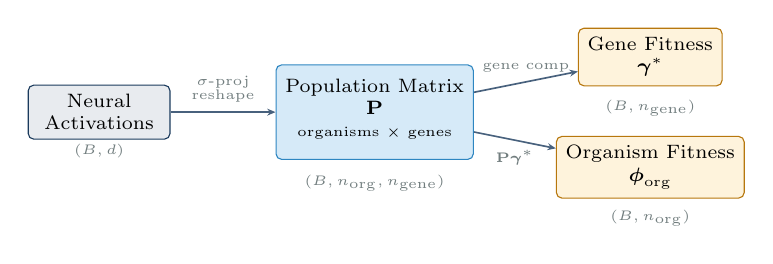
\begin{tikzpicture}[
  databox/.style  = {draw=primary, fill=primary!10, rounded corners=2pt, minimum width=1.8cm, minimum height=0.6cm, align=center, font=\scriptsize},
  popbox/.style   = {draw=accent, fill=accentlight, rounded corners=2pt, minimum width=2.2cm, minimum height=1.2cm, align=center, font=\scriptsize},
  fitbox/.style   = {draw=learned, fill=learnedlight, rounded corners=2pt, minimum width=1.8cm, minimum height=0.6cm, align=center, font=\scriptsize},
  arr/.style      = {-{Stealth[length=3pt,width=2.5pt]}, semithick, color=primary!80},
  lbl/.style      = {font=\tiny, color=muted},
]
\node[databox] (data) at (0, 0) {Neural\\Activations};
\node[lbl] at (0, -0.5) {$(B, d)$};
\node[popbox] (pop) at (3.5, 0) {Population Matrix\\$\mathbf{P}$\\\vspace{2pt}\tiny organisms $\times$ genes};
\node[lbl] at (3.5, -0.9) {$(B, n_\mathrm{org}, n_\mathrm{gene})$};
\node[fitbox] (gfit) at (7.0, 0.7) {Gene Fitness\\$\boldsymbol{\gamma}^*$};
\node[lbl] at (7.0, 0.05) {$(B, n_\mathrm{gene})$};
\node[fitbox] (ofit) at (7.0, -0.7) {Organism Fitness\\$\boldsymbol{\phi}_\mathrm{org}$};
\node[lbl] at (7.0, -1.35) {$(B, n_\mathrm{org})$};
\draw[arr] (data) -- node[above, font=\tiny, color=muted, align=center] {$\sigma$-proj\\[-1pt]\tiny reshape} (pop);
\draw[arr] (pop) -- node[above, font=\tiny, color=muted] {gene comp} (gfit);
\draw[arr] (pop) -- node[below, font=\tiny, color=muted] {$\mathbf{P}\boldsymbol{\gamma}^*$} (ofit);
\end{tikzpicture}
\caption{Genetic AI transforms neural activations into a population matrix where rows represent organisms (latent feature groups within each sample) and columns represent genes (latent dimensions). For each sample in the batch, a separate population matrix is created. Fixed-formula fitness computations yield gene fitness through relative competition and organism fitness through weighted gene expression.}
\label{fig:genetic_concept}
\end{figure}

\begin{figure*}[!t]
\centering
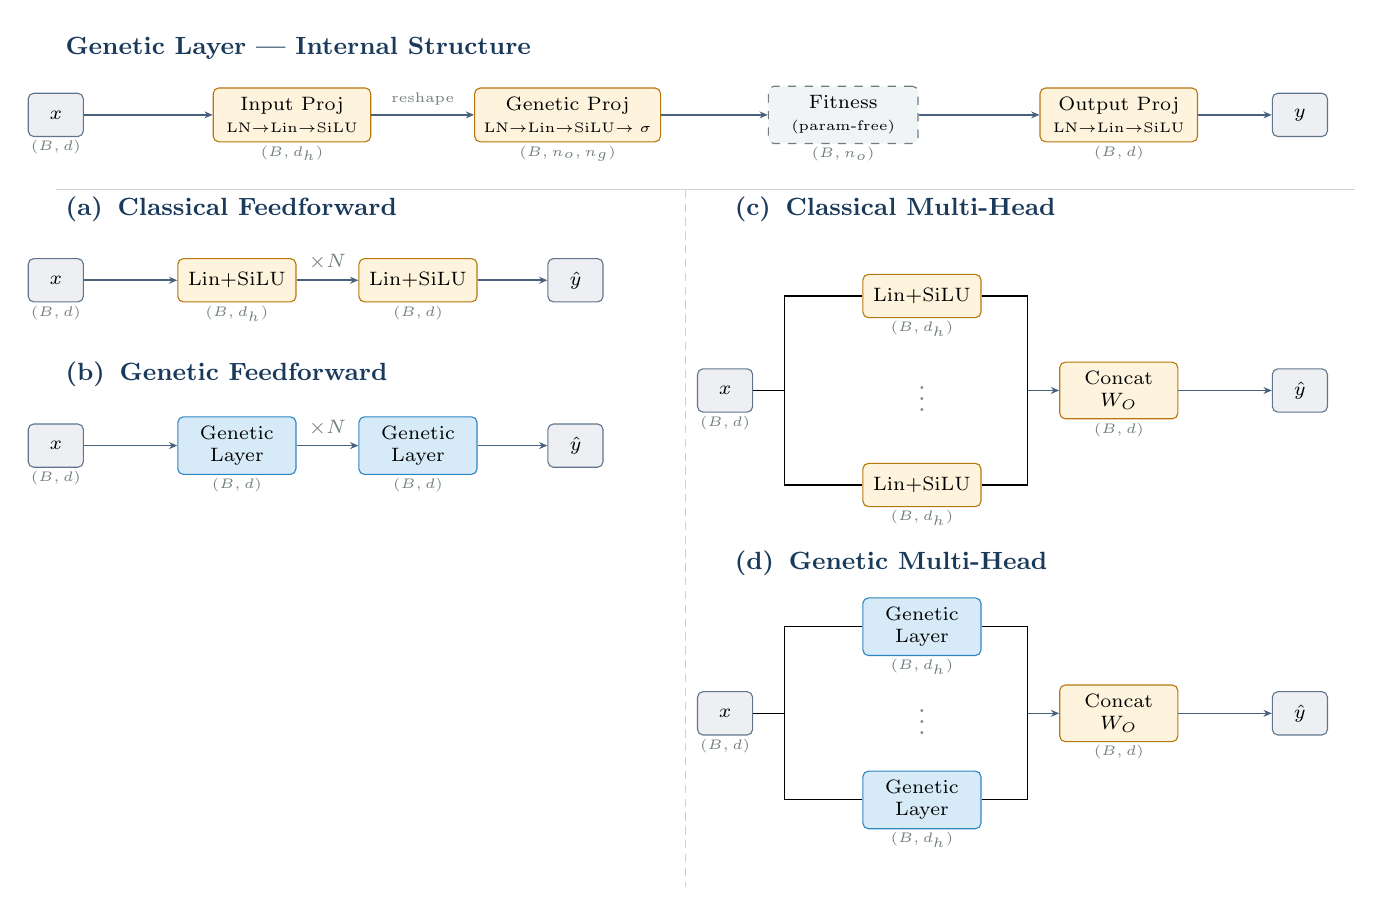
\begin{tikzpicture}[
  gbox/.style  = {draw=accent, fill=accentlight, rounded corners=2pt, minimum width=1.5cm, minimum height=0.55cm, align=center, font=\scriptsize},
  lbox/.style  = {draw=learned, fill=learnedlight, rounded corners=2pt, minimum width=1.5cm, minimum height=0.55cm, align=center, font=\scriptsize},
  pbox/.style  = {draw=muted, fill=highlight, dashed, rounded corners=2pt, minimum width=1.9cm, minimum height=0.55cm, align=center, font=\scriptsize},
  iobox/.style = {draw=primary!70, fill=primary!8, rounded corners=2pt, minimum width=0.7cm, minimum height=0.55cm, align=center, font=\scriptsize},
  arr/.style   = {-{Stealth[length=3pt,width=2.5pt]}, semithick, color=primary!80},
  lbl/.style   = {font=\tiny, color=muted, anchor=north, inner sep=1pt},
]
%%--- Genetic Layer: Internal Structure (full width) ---
\node[font=\small\bfseries\color{primary}, anchor=west] at (0, 0.85) {Genetic Layer --- Internal Structure};
\node[iobox] (gx)  at (0,    0) {$x$};
\node[lbox, minimum width=2.0cm]  (gip) at (3.0,  0) {Input Proj\\{\tiny LN$\to$Lin$\to$SiLU}};
\node[lbox, minimum width=2.3cm]  (ggp) at (6.5,  0) {Genetic Proj\\{\tiny LN$\to$Lin$\to$SiLU$\to\sigma$}};
\node[pbox]                       (gf)  at (10.0, 0) {Fitness\\{\tiny (param-free)}};
\node[lbox, minimum width=2.0cm]  (gop) at (13.5, 0) {Output Proj\\{\tiny LN$\to$Lin$\to$SiLU}};
\node[iobox] (gy)  at (15.8, 0) {$y$};
\draw[arr] (gx)--(gip); \draw[arr] (gip)-- node[above, font=\tiny, color=muted] {reshape} (ggp); \draw[arr] (ggp)--(gf); \draw[arr] (gf)--(gop); \draw[arr] (gop)--(gy);
\node[lbl] at (gx.south)  {$(B,d)$};
\node[lbl] at (gip.south) {$(B,d_h)$};
\node[lbl] at (ggp.south) {$(B,n_o,n_g)$};
\node[lbl] at (gf.south)  {$(B,n_o)$};
\node[lbl] at (gop.south) {$(B,d)$};
%%--- Horizontal rule ---
\draw[color=muted!35, thin] (0, -0.95) -- (16.5, -0.95);
%%--- (a) Classical Feedforward ---
\node[font=\small\bfseries\color{primary}, anchor=west] at (0, -1.2) {(a)\enspace Classical Feedforward};
\node[iobox] (ax)  at (0,   -2.1) {$x$};
\node[lbox]  (al1) at (2.3, -2.1) {Lin$+$SiLU};
\node[lbox]  (al2) at (4.6, -2.1) {Lin$+$SiLU};
\node[iobox] (ay)  at (6.6, -2.1) {$\hat{y}$};
\draw[arr] (ax)--(al1); \draw[arr] (al1)--(al2) node[midway, above, font=\scriptsize, color=muted] {$\times N$}; \draw[arr] (al2)--(ay);
\node[lbl] at (ax.south)  {$(B,d)$};
\node[lbl] at (al1.south) {$(B,d_h)$};
\node[lbl] at (al2.south) {$(B,d)$};
%%--- (b) Genetic Feedforward ---
\node[font=\small\bfseries\color{primary}, anchor=west] at (0, -3.3) {(b)\enspace Genetic Feedforward};
\node[iobox] (bx)  at (0,   -4.2) {$x$};
\node[gbox]  (bg1) at (2.3, -4.2) {Genetic\\Layer};
\node[gbox]  (bg2) at (4.6, -4.2) {Genetic\\Layer};
\node[iobox] (by)  at (6.6, -4.2) {$\hat{y}$};
\draw[arr] (bx)--(bg1); \draw[arr] (bg1)--(bg2) node[midway, above, font=\scriptsize, color=muted] {$\times N$}; \draw[arr] (bg2)--(by);
\node[lbl] at (bx.south)  {$(B,d)$};
\node[lbl] at (bg1.south) {$(B,d)$};
\node[lbl] at (bg2.south) {$(B,d)$};
%%--- Vertical divider ---
\draw[color=muted!35, densely dashed, thin] (8.0, -0.95) -- (8.0, -9.8);
%%--- (c) Classical Multi-Head ---
%% heads at y = -2.3, -3.5, -4.7 (pitch 1.2); cx/ccat/cy centred at -3.5
\node[font=\small\bfseries\color{primary}, anchor=west] at (8.5, -1.2) {(c)\enspace Classical Multi-Head};
\node[iobox] (cx)   at (8.5,  -3.5) {$x$};
\node[lbox]  (ch1)  at (11.0, -2.3) {Lin$+$SiLU};
\node[font=\normalsize, color=primary!60] (cvdots) at (11.0, -3.5) {$\vdots$};
\node[lbox]  (ch3)  at (11.0, -4.7) {Lin$+$SiLU};
\node[lbox]  (ccat) at (13.5, -3.5) {Concat\\$W_O$};
\node[iobox] (cy)   at (15.8, -3.5) {$\hat{y}$};
\coordinate (cfork) at ($(cx.east)+(0.4,0)$);
\coordinate (cjoin) at ($(ccat.west)+(-0.4,0)$);
\draw (cx.east)--(cfork); \draw (cfork)|-(ch1.west); \draw (cfork)|-(ch3.west);
\draw (ch1.east)-|(cjoin); \draw (ch3.east)-|(cjoin);
\draw[arr] (cjoin)--(ccat.west); \draw[arr] (ccat)--(cy);
\node[lbl] at (cx.south)   {$(B,d)$};
\node[lbl] at (ch1.south)  {$(B,d_h)$};
\node[lbl] at (ch3.south)  {$(B,d_h)$};
\node[lbl] at (ccat.south) {$(B,d)$};
%%--- (d) Genetic Multi-Head ---
%% heads at y = -6.5, -7.6, -8.7 (pitch 1.1); dx/dcat/dy centred at -7.6
%% title at -5.7 leaves > 0.5 gap above dh1 top edge
\node[font=\small\bfseries\color{primary}, anchor=west] at (8.5, -5.7) {(d)\enspace Genetic Multi-Head};
\node[iobox] (dx)   at (8.5,  -7.6) {$x$};
\node[gbox]  (dh1)  at (11.0, -6.5) {Genetic\\Layer};
\node[font=\normalsize, color=primary!60] (dvdots) at (11.0, -7.6) {$\vdots$};
\node[gbox]  (dh3)  at (11.0, -8.7) {Genetic\\Layer};
\node[lbox]  (dcat) at (13.5, -7.6) {Concat\\$W_O$};
\node[iobox] (dy)   at (15.8, -7.6) {$\hat{y}$};
\coordinate (dfork) at ($(dx.east)+(0.4,0)$);
\coordinate (djoin) at ($(dcat.west)+(-0.4,0)$);
\draw (dx.east)--(dfork); \draw (dfork)|-(dh1.west); \draw (dfork)|-(dh3.west);
\draw (dh1.east)-|(djoin); \draw (dh3.east)-|(djoin);
\draw[arr] (djoin)--(dcat.west); \draw[arr] (dcat)--(dy);
\node[lbl] at (dx.south)   {$(B,d)$};
\node[lbl] at (dh1.south)  {$(B,d_h)$};
\node[lbl] at (dh3.south)  {$(B,d_h)$};
\node[lbl] at (dcat.south) {$(B,d)$};
\end{tikzpicture}
\caption{\emph{Top}: internal structure of a Genetic Layer (Section~\ref{sec:layers}). Amber boxes are learned projections (LayerNorm $\to$ Linear $\to$ SiLU); dashed grey box is the parameter-free fitness computation. The Genetic Projection outputs a flat vector that is reshaped into the population matrix structure. \emph{Bottom}: the four topology variants evaluated in Experiment~I. Amber boxes are all learned blocks (linear layers and output projections); blue boxes are Genetic Layer modules (each expands $(B,d)\!\to\!(B,n_o,n_g)\!\to\!(B,n_o)$ then projects back to $(B,d)$). Labels show output tensor shape ($B$ = batch, $d$ = feature dim, $d_h$ = head/hidden dim, $n_o$ = organisms, $n_g$ = genes).}
\label{fig:arch_exp1}
\end{figure*}

% ============================================================
\section{Experiment I: Genetic Layers}
\label{sec:layers}
% ============================================================

\subsection*{Background}

A standard feedforward layer maps input $\mathbf{x}\in\mathbb{R}^{d_\mathrm{in}}$ through a learned linear transformation followed by a non-linearity $\sigma$:
%
\begin{equation*}
  \mathbf{h} = \sigma(W\mathbf{x} + \mathbf{b}), \qquad W\in\mathbb{R}^{d_\mathrm{out}\times d_\mathrm{in}},\;\mathbf{b}\in\mathbb{R}^{d_\mathrm{out}}.
\end{equation*}
%
A multi-head network runs $K$ independent heads in parallel and concatenates their outputs via an output projection $W_O$:
%
\begin{equation*}
  \mathrm{MH}(\mathbf{x}) = \bigl[\mathbf{h}_1(\mathbf{x})\;\|\;\cdots\;\|\;\mathbf{h}_K(\mathbf{x})\bigr]W_O.
\end{equation*}
%
This experiment replaces classical linear transformations with \textsf{GeneticLayer} modules that sandwich the parameter-free fitness computation between learned projections. An input projection (LayerNorm $\to$ Linear $\to$ SiLU) maps the input to a hidden dimension. A genetic projection (LayerNorm $\to$ Linear $\to$ SiLU $\to\sigma$) maps that to the population matrix $\mathbf{P}\in[0,1]^{n_\mathrm{org}\times n_\mathrm{gene}}$. Fitness is then computed via Eqs.~\eqref{eq:genemean}--\eqref{eq:orgfitness}, and an output projection maps organism fitness scores to the target dimension. Figure~\ref{fig:arch_exp1} shows the internal structure and the four topology variants.

\subsection*{Setup}

This experiment evaluates genetic layers as substitutes for learned linear transformations on seven tabular classification benchmarks. We replace the linear layers in two standard network topologies with hybrid \emph{genetic layers}: each layer projects its input to a population matrix via a sigmoid, applies the fitness computation of Eqs.~(1)--(3), and returns the organism fitness vector. The surrounding projection weights are trained with Adam; the fitness computation itself is parameter-free. Seven tabular datasets are used (Iris, Wine, Breast Cancer, Digits, Synthetic, CovType, Olivetti Faces), spanning 4 to 4,096 features. For CovType, a 10,000-sample subset of the full 581K-sample dataset was used. Two topologies are evaluated: \emph{feedforward} stacks (depths 2, 4, 6) and \emph{parallel heads} (1, 2, 3 heads concatenated). All configurations: 128 epochs, Adam optimiser, batch size 16,384. The evaluation metric is balanced accuracy.

\subsection*{Results}

\begin{table}[ht]
  \small
  \centering
  \caption{Average performance across all seven datasets.}
  \label{tab:layer_summary}
  \setlength{\tabcolsep}{5pt}
  \begin{tabularx}{\linewidth}{@{}X X r r@{}}
    \toprule
    \textbf{Topology} & \textbf{Type} & \textbf{Bal.\ Acc.} & \textbf{Params} \\
    \midrule
    Feedforward & Classical & 88.7\%          & 48,851 \\
    Feedforward & Genetic   & 49.1\%          & 25,667 \\
    Heads       & Classical & 79.5\%          & 41,330 \\
    Heads       & Genetic   & \textbf{80.8\%} & 44,235 \\
    \bottomrule
  \end{tabularx}
\end{table}

The topological split is stark and consistent. Genetic feedforward networks underperform by 39.6 percentage points on average and, crucially, \emph{degrade with depth}. On Digits, accuracy falls from 53.0\% at depth~2 to 29.4\% at depth~4 and 18.8\% at depth~6 --- the inverse of the classical trend (94.8\%, 97.2\%, 97.5\%). The same pattern holds on every high-dimensional dataset. Because Eq.~\eqref{eq:genefitness} is a fixed-formula transformation, stacking multiple such layers does not build abstraction; it compounds information loss at each stage.

Genetic multi-head networks outperform classical heads on average (80.8\% vs.\ 79.5\%) and scale better with head count. Classical networks show only moderate improvement from 1 to 3 heads; genetic networks improve substantially. Table~\ref{tab:layer_wins} shows the three datasets with the largest genetic advantage.

\begin{table}[ht]
  \small
  \centering
  \caption{Datasets where genetic heads most exceed classical heads (best genetic head count vs.\ best classical head count).}
  \label{tab:layer_wins}
  \setlength{\tabcolsep}{4pt}
  \begin{tabularx}{\linewidth}{@{}X r r r@{}}
    \toprule
    \textbf{Dataset} & \textbf{Genetic} & \textbf{Classical} & $\Delta$ \\
    \midrule
    Synthetic (50 feat.) & 59.6\% & 47.6\% & +12.0pp \\
    CovType   (54 feat.) & 75.0\% & 66.6\% & \phantom{0}+8.4pp \\
    Digits    (64 feat.) & 97.6\% & 94.8\% & \phantom{0}+2.8pp \\
    \bottomrule
  \end{tabularx}
\end{table}

We speculate that parallel genetic heads succeed because each head maps the input to a distinct population matrix $\mathbf{P}$, inducing an ensemble of complementary fitness landscapes. The three top-performing datasets share medium feature dimensionality (50--64) and multi-class output structure (7, 7, and 10 classes). By contrast, a single deep stack repeatedly applies the same fixed-formula transformation and compounds information loss toward a fixed-point.

Parameter efficiency is competitive in the multi-head setting: genetic heads use only 7\% more parameters than classical on average, compared to 48\% \emph{fewer} for genetic feedforward (which achieves far less accuracy). Training overhead is notable: 17\% slower for genetic heads and 27\% slower for genetic feedforward.

\subsection*{Limitations}

These are preliminary results. Each configuration used a single fixed train/test split (80/20, \texttt{random\_state=8080}), with no cross-validation or repeated runs. For small datasets such as Iris ($n{=}150$) and Wine ($n{=}178$), a single split can yield high-variance estimates, and reported differences may not survive a change of seed. The depth-degradation finding is consistent across all seven datasets and likely robust. The per-dataset multi-head figures in Table~\ref{tab:layer_wins} are indicative only.

\subsection*{Key Takeaway}

\begin{tcolorbox}[resultbox]
  \small Genetic AI hybridisation is \textbf{topology-sensitive}: it fails in sequential depth stacks and succeeds in parallel multi-head configurations. Hybrid multi-head networks match or outperform fully-learned counterparts on several medium-dimensional multi-class benchmarks at a comparable parameter budget.
\end{tcolorbox}

% ============================================================
\section{Experiment II: Genetic Attention}
\label{sec:attention}
% ============================================================

\subsection*{Background}

\Ac{mha}~\cite{vaswani2017attention} maps the input $X\in\mathbb{R}^{B\times T\times d}$ (batch~$B$, sequence length~$T$, hidden size~$d$) to queries, keys, and values $Q,K,V\in\mathbb{R}^{B\times T\times d_k}$ via learned projections $W^Q, W^K, W^V\in\mathbb{R}^{d\times d_k}$, with $d_k=d/h$ for $h$ heads:
%
\begin{equation*}
  Q = XW^Q, \quad K = XW^K, \quad V = XW^V.
\end{equation*}
%
The attention output is the value-weighted sum over all positions, with weights derived from scaled query--key similarity:
%
\begin{equation*}
  \mathrm{Attn}(Q,K,V) = \mathrm{softmax}\!\left(\tfrac{QK^\top}{\sqrt{d_k}}\right)V.
\end{equation*}
%
All projection matrices are fully learned. The parallel-head success in Experiment~I motivates asking whether a genetic prior on the value pathway can improve retrieval, keeping the QK similarity computation intact.

\subsection*{Design}

Initial decoder designs explored two strategies for injecting genetic fitness into attention:

\begin{itemize}[leftmargin=1.5em, itemsep=2pt, topsep=2pt]
  \item \textbf{Value-only}: Q and K are eliminated. The value matrix $V\in\mathbb{R}^{B\times h\times T\times d_k}$, scaled to $[0,1]$, is used directly as the population matrix $\mathbf{P}$ (organisms $=$ tokens, genes $=$ $d_k$ head features). Eqs.~\eqref{eq:genemean}--\eqref{eq:genefitness} yield gene fitness $\boldsymbol{\gamma}^*\in\mathbb{R}^{d_k}$; the score $\phi_{ij}=V_j\cdot\boldsymbol{\gamma}^*_i$ replaces the usual $Q_i\cdot K_j$ similarity.
  \item \textbf{Score-matrix modulation}: a $T\!\times\!T$ score matrix $S$ is constructed (either from dedicated projections $O'G'{}^\top/\sqrt{d_k}$ replacing QK entirely, or as $\sigma(QK^\top/\sqrt{d_k})$ on top of the standard path). $S$ is used as the population matrix (organisms $=$ query tokens, genes $=$ key tokens); Eqs.~\eqref{eq:genemean}--\eqref{eq:orgfitness} yield per-token organism fitness $\boldsymbol{\phi}_\mathrm{org}\in\mathbb{R}^T$, which re-weights the rows of $S$ before softmax and multiplication by $V$.
\end{itemize}

Neither approach converged reliably in the decoder setting. Two compounding failure modes were identified:

\textbf{Statistical instability.} The gene-mean computation (Eq.~\eqref{eq:genemean}) estimates each gene's typical expression level by averaging normalised value activations across all sequence positions. In a decoder with causal masking, position~$t$ can only see positions $1,\ldots,t$, so early tokens average over just one or two values, which is an extremely noisy estimate. Because each position sees a different prefix length, $\tilde{\Phi}_g$ is also asymmetric across positions, making it an unstable learning signal during early training. The genetic prior is intended to be a stable structural signal; in the causal setting it becomes a moving, position-dependent quantity.

\textbf{Computational cost.} A correct causal implementation cannot compute a single shared gene-fitness vector per forward pass. To preserve causality, the fitness computation must be run separately for each prefix length $t = 1, \ldots, T$, producing $T$ independent $\boldsymbol{\gamma}^*$ vectors before the attention output at any position can be formed. This makes the per-step cost scale as $O(T)$ gene-fitness evaluations rather than one, an overhead that compounds the instability problem and makes training impractically slow at even moderate sequence lengths.

\subsection*{Final Design}

Both failure modes trace back to a fundamental structural mismatch: the gene-mean computation requires a stable average over \emph{all} visible positions, but causal masking makes that set grow with each token, rendering the mean noisy and position-dependent. The genetic prior is therefore better suited to \emph{non-causal} (bidirectional) attention, where every position sees the full sequence and $\tilde{\Phi}_g$ is stable. We therefore applied the design to a \acs{bert}-style encoder, keeping the standard Q--K path intact and applying the genetic prior only to $V$. Unlike the Genetic Layer (Figure~\ref{fig:arch_exp1}), which adds dedicated projections around the fitness computation, this approach applies fitness directly to the value matrix $V$ produced by standard attention, without introducing new parameters. We call the resulting mechanism \ac{mga}:
%
\begin{align}
  V_\mathrm{norm} &= \sigma(V), \\[2pt]
  \tilde{\Phi}_g  &= \frac{1}{T}\sum_{t=1}^{T}
                     V_\mathrm{norm}[:, :, t, g], \\[2pt]
  \gamma_g^*      &= \left(\sum_{s=1}^{d}
                     \frac{\tilde{\Phi}_g + \tfrac{1}{2}}
                          {\tilde{\Phi}_s + \tfrac{1}{2}}\right)^{-1}\!\!, \\[2pt]
  V_\mathrm{gen}  &= V \odot \boldsymbol{\gamma}^*,
\end{align}
%
\begin{equation}
  \mathrm{MGA}(Q,K,V)
    = \mathrm{softmax}\!\left(\tfrac{QK^\top}{\sqrt{d}}\right)V_\mathrm{gen}.
  \label{eq:mga}
\end{equation}
%
This modulates \emph{which features} the attention output emphasises, without altering \emph{which positions} it weights. The fitness $\boldsymbol{\gamma}^*$ is computed fresh for each forward pass from the value activations of the current batch, making it input-dependent and parameter-free beyond the existing value projection weights.

\subsection*{Setup}

A six-layer \acs{bert}~\cite{devlin2019bert} (hidden size 384, 12 attention heads, $d_\mathrm{head}=32$, intermediate size 1,536) is trained as a dual encoder~\cite{karpukhin2020dpr} for passage retrieval on MS-MARCO~\cite{bajaj2016msmarco} (503K training pairs, 101K test pairs). Query and passage encoders share the same backbone. Sentence representations are obtained by mean pooling over valid tokens and L2-normalising. Training uses InfoNCE loss with in-batch negatives (batch size 512), AdamW with linear warmup, fixed seed 8080, for 2048 steps.

\begin{figure*}[tp]
  \centering
  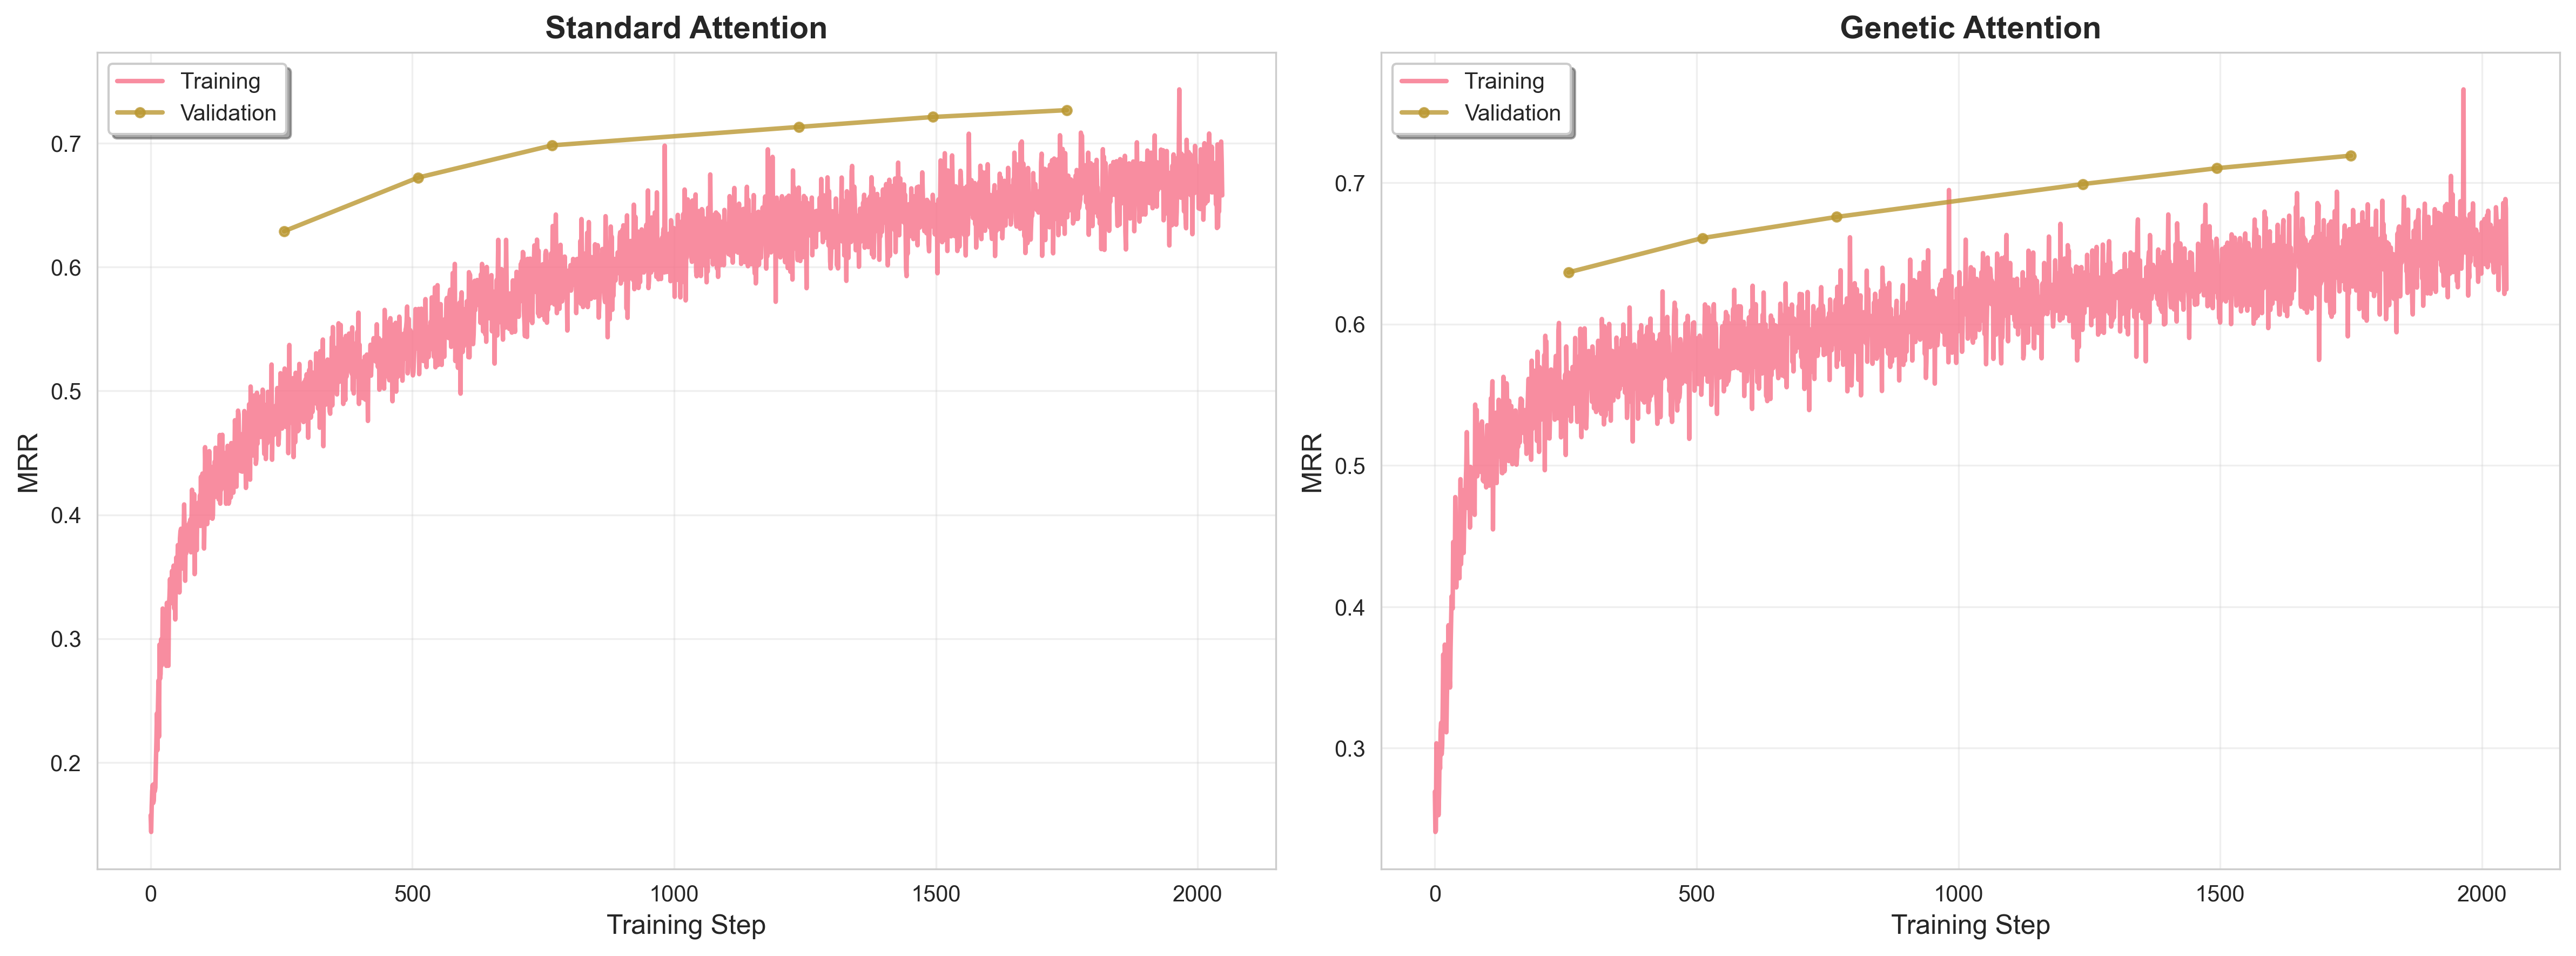
\includegraphics[width=\linewidth]
    {../genetic_attention/artefacts/mrr_comparison.png}
  \caption{\Ac{mrr} over training steps. Genetic attention leads early before being overtaken by the standard baseline, which continues improving to convergence.}
  \label{fig:mrr}
\end{figure*}

\subsection*{Results}

\begin{table}[ht]
  \small
  \centering
  \caption{MS-MARCO dual-encoder results at 2,048 training steps.}
  \label{tab:attn_results}
  \setlength{\tabcolsep}{4pt}
  \begin{tabularx}{\linewidth}{@{}X r r r r@{}}
    \toprule
    \textbf{Config} & \textbf{\acs{mrr}} & \textbf{\acs{ndcg}@5}
      & \textbf{Hit@5} & \textbf{Time (s)} \\
    \midrule
    Standard & 0.492 & 0.500 & 0.573 & \phantom{0}7,822 \\
    Genetic  & 0.486 & 0.492 & 0.568 & 11,947 \\
    \midrule
    $\Delta$ & $-1.2\%$ & $-1.6\%$ & $-0.9\%$ & $+52.8\%$ \\
    \bottomrule
  \end{tabularx}
\end{table}

At 2,048 steps, standard attention outperforms genetic attention across all retrieval metrics. The training curves (Figure~\ref{fig:mrr}) show an early-training reversal: genetic attention \emph{leads} during the first several hundred steps before the standard baseline overtakes it and continues to improve. This is consistent with $\boldsymbol{\gamma}^*$ acting as an initialisation prior. Once the value projections are sufficiently trained, unconstrained attention has greater capacity and the fixed modulation becomes a ceiling.


The 52.8\% training overhead arises because $\boldsymbol{\gamma}^*$ is not a fixed parameter: it is derived from the value activations of the current batch on every forward pass. Concretely, Eqs.~\eqref{eq:genemean}--\eqref{eq:genefitness} run as an extra sequential step after every value projection.

\subsection*{Limitations}

These results should be treated as preliminary: one seed, one run per configuration, and a 2,048-step budget. No repeated runs, hyperparameter sweeps, or significance testing were performed. A rigorous comparison would require multiple seeds, runs to full convergence, and paired statistical tests. The reported metric differences ($\leq$1.6 percentage points) are within a range explainable by seed variance alone.

\begin{tcolorbox}[resultbox]
  \small Hybridising attention with a genetic value prior provides an \textbf{early-training advantage} in retrieval metrics but is overtaken at convergence. Fully-learned attention achieves lower validation loss and better test metrics with 35\% less training time.
\end{tcolorbox}

% ============================================================
\section{Future Directions}
\label{sec:future}
% ============================================================

\begin{figure}[t]
\centering
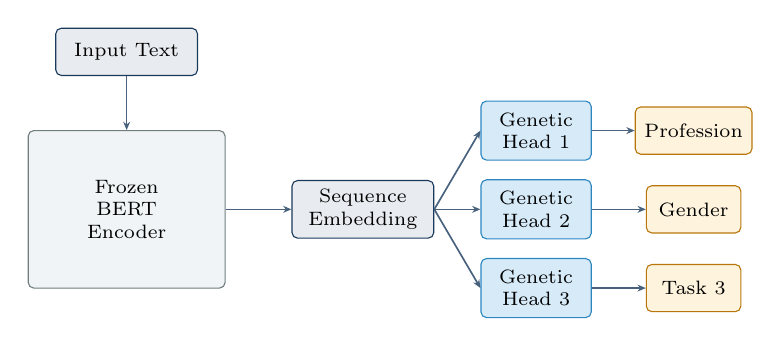
\begin{tikzpicture}[
  encbox/.style = {draw=muted, fill=highlight, rounded corners=2pt, minimum width=2.5cm, minimum height=2.0cm, align=center, font=\scriptsize},
  ghead/.style  = {draw=accent, fill=accentlight, rounded corners=2pt, minimum width=1.4cm, minimum height=0.75cm, align=center, font=\scriptsize},
  outbox/.style = {draw=learned, fill=learnedlight, rounded corners=2pt, minimum width=1.2cm, minimum height=0.6cm, align=center, font=\scriptsize},
  inpbox/.style = {draw=primary, fill=primary!10, rounded corners=2pt, minimum width=1.8cm, minimum height=0.6cm, align=center, font=\scriptsize},
  arr/.style    = {-{Stealth[length=3pt,width=2.5pt]}, semithick, color=primary!80},
  lbl/.style    = {font=\tiny, color=muted},
]
\node[inpbox] (inp) at (0, 2.0) {Input Text};
\node[encbox] (bert) at (0, 0) {Frozen\\BERT\\Encoder};
\node[inpbox] (cls) at (3.0, 0) {Sequence\\Embedding};
\node[ghead] (h1) at (5.2, 1.0) {Genetic\\Head 1};
\node[ghead] (h2) at (5.2, 0) {Genetic\\Head 2};
\node[ghead] (h3) at (5.2, -1.0) {Genetic\\Head 3};
\node[outbox] (out1) at (7.2, 1.0) {Profession};
\node[outbox] (out2) at (7.2, 0) {Gender};
\node[outbox] (out3) at (7.2, -1.0) {Task 3};
\draw[arr] (inp.south) -- (bert.north);
\draw[arr] (bert.east) -- (cls.west);
\draw[arr] (cls.east) -- (h1.west);
\draw[arr] (cls.east) -- (h2.west);
\draw[arr] (cls.east) -- (h3.west);
\draw[arr] (h1.east) -- (out1.west);
\draw[arr] (h2.east) -- (out2.west);
\draw[arr] (h3.east) -- (out3.west);
\end{tikzpicture}
\caption{Proposed Genetic Adapter architecture: independent genetic heads on a frozen encoder partition fitness landscapes by task.}
\label{fig:genetic_adapter}
\end{figure}

\subsection*{Experiment III: Genetic Adapter}

We propose attaching a genetic multi-head module to a frozen \acs{bert} encoder as a lightweight classification adapter, motivated by the multi-head gains in Experiment~I. The evaluation target is the Bias-in-Bios dataset~\cite{biasinbios} (biography text, profession and gender labels). The multi-task structure tests whether independent genetic heads partition fitness landscapes by task. Counterfactual pronoun-swapping would additionally test whether genetic competition incidentally reduces gender bias. Figure~\ref{fig:genetic_adapter} shows the proposed architecture.

\subsection*{Experiment IV: Genetic Expert Routing in \acs{moe}}

We propose replacing the learned router in \acs{moe} architectures~\cite{shazeer2017moe} with a genetic fitness computation: each expert is treated as an organism, each token's feature dimensions as genes, and the top-$k$ experts are selected by organism fitness~\eqref{eq:orgfitness}. This yields a parameter-free routing mechanism analogous to the multi-head ensemble effect in Experiment~I, and may avoid the load-balancing instabilities of learned routers. Validating this requires at least $\sim$1B parameter models and is deferred to higher-compute settings. Figure~\ref{fig:genetic_moe} illustrates the proposed routing mechanism.

\begin{figure}[H]
\centering
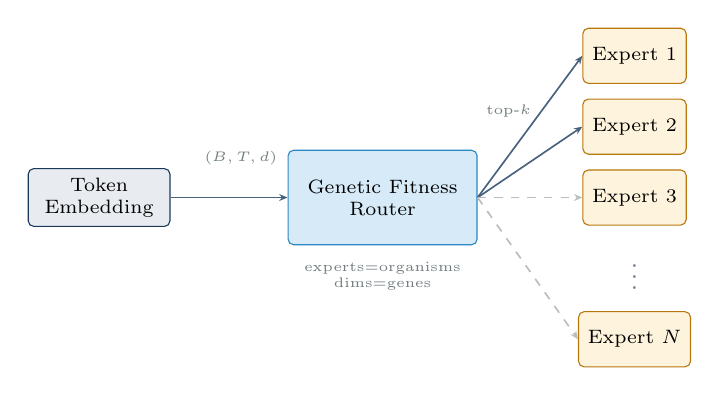
\begin{tikzpicture}[
  tokbox/.style = {draw=primary, fill=primary!10, rounded corners=2pt, minimum width=1.8cm, minimum height=0.7cm, align=center, font=\scriptsize},
  routbox/.style = {draw=accent, fill=accentlight, rounded corners=2pt, minimum width=2.4cm, minimum height=1.2cm, align=center, font=\scriptsize},
  expbox/.style = {draw=learned, fill=learnedlight, rounded corners=2pt, minimum width=1.2cm, minimum height=0.7cm, align=center, font=\scriptsize},
  arr/.style = {-{Stealth[length=3pt,width=2.5pt]}, semithick, color=primary!80},
  arrdash/.style = {-{Stealth[length=3pt,width=2.5pt]}, semithick, color=muted!50, dashed},
  lbl/.style = {font=\tiny, color=muted},
]
\node[tokbox] (tok) at (0, 0) {Token\\Embedding};
\node[lbl] at (1.8, 0.5) {$(B,T,d)$};
\node[routbox] (rout) at (3.6, 0) {Genetic Fitness\\Router};
\node[lbl, align=center] at (3.6, -1.0) {experts=organisms\\dims=genes};
\node[expbox] (e1) at (6.8, 1.8) {Expert 1};
\node[expbox] (e2) at (6.8, 0.9) {Expert 2};
\node[expbox] (e3) at (6.8, 0) {Expert 3};
\node[font=\normalsize, color=primary!60] at (6.8, -0.9) {$\vdots$};
\node[expbox] (en) at (6.8, -1.8) {Expert $N$};
\node[lbl] at (5.2, 1.1) {top-$k$};
\draw[arr] (tok.east) -- (rout.west);
\draw[arr] (rout.east) -- (e1.west);
\draw[arr] (rout.east) -- (e2.west);
\draw[arrdash] (rout.east) -- (e3.west);
\draw[arrdash] (rout.east) -- (en.west);
\end{tikzpicture}
\caption{Proposed Genetic \acs{moe} architecture: organism fitness scores replace learned routing. Top-$k$ selection by fitness provides parameter-free, diversity-preserving routing.}
\label{fig:genetic_moe}
\end{figure}

% ============================================================
\section{Conclusion}
% ============================================================

The two completed experiments establish a clear boundary condition for Genetic AI hybridisation with machine learning. First, hybridisation is \emph{topology-sensitive}: inserting the genetic prior into sequential depth stacks compounds information loss at each fixed-formula stage, causing performance to degrade monotonically with depth. By contrast, parallel multi-head architectures benefit from the genetic prior because each head converges to a distinct fitness equilibrium, producing a complementary ensemble. Second, genetic priors \emph{accelerate early training but saturate}: genetic value modulation leads retrieval metrics early before the unconstrained baseline catches up at convergence.

The genetic prior is most useful when \emph{diversity is incentivised} (parallel independent heads) and \emph{training is short} (warm-up or cold-start settings). It becomes a constraint in sequential stacks and long fine-tuning runs, where the fixed formula limits capacity. The proposed Genetic Adapter and Genetic \acs{moe} experiments target larger scale and more complex task structure, to test whether gains extend beyond the early-training window.

Code and results are available in danube.ai's open-source repository: \url{https://github.com/danube-ai/pikaia}.

% ============================================================
\clearpage
\onecolumn
\section*{Acronyms}
\acuse{bert}\acuse{ndcg}
\printacronyms[heading=none]
\clearpage
\bibliographystyle{plain}
\bibliography{references}
% ============================================================

\end{document}
